\documentclass[../cnd.tex]{subfiles}

Khái niệm "Ethereum"  có thể được sử dụng để chỉ ba thứ khác nhau: giao thức Ethereum, mạng Ethereum, và dự án Ethereum bao gồm cả hai thứ trên. Có thể thấy sức mạnh chủ yếu của nó đến từ giao thức. 

 Ethereum là một nền tảng điện toán có tính chất phân tán, công cộng, mã nguồn mở dựa trên công nghệ chuỗi khối. Nó có tính năng hợp đồng thông minh (smart contracts), tạo thuận lợi cho các thỏa thuận hợp đồng trực tuyến.$^{[6]}$
		
\subsubsection{Lịch sử ra đời}

\begin{figure}[ht]
	\centering
	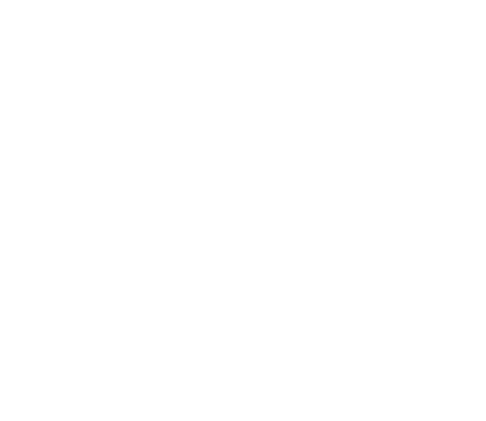
\includegraphics[width=0.8\linewidth]{../img/logo}
	\caption{Logo Ethereum}
	\label{fig:logo}
\end{figure}

Ethereum ban đầu được mô tả trong một văn bản của Vitalik Buterin, một lập trình viên liên quan đến Bitcoin vào cuối năm 2013 với mục tiêu xây dựng các ứng dụng phân quyền. Buterin đã lập luận rằng Bitcoin cần một ngôn ngữ kịch bản để phát triển ứng dụng. Không đạt được thỏa thuận với nhóm phát triển Bitcoin, ông đề xuất phát triển một nền tảng mới với một ngôn ngữ kịch bản tổng quát hơn.

 Bốn thành viên ban đầu của nhóm Ethereum là Vitalik Buterin, Mihai Alisie, Anthony Di Iorio và Charles Hoskinson. Phát triển chính thức của dự án phần mềm Ethereum bắt đầu vào đầu năm 2014 thông qua một công ty Thụy Sĩ tên là Ethereum Switzerland GmbH (EthSuisse). Sau đó, một tổ chức phi lợi nhuận tại Thụy Sĩ với tên gọi là Ethereum Foundation cũng được thành lập. Việc phát triển Ethereum được tài trợ bởi đám đông trực tuyến trong suốt tháng 7 và tháng 8 năm 2014, với những người tham gia mua Ethereum bằng các loại tiền kỹ thuật số khác như bitcoin. Mặc dù đã có những lời khen ngợi đầu tiên về những đổi mới kỹ thuật của Ethereum, nhưng cũng có các ngờ vực về tính an toàn và khả năng mở rộng của nó.
		